\documentclass[12pt,a4paper]{article}
\usepackage[utf8]{inputenc}
\usepackage[T2A]{fontenc}
\usepackage[ukrainian]{babel}
\usepackage{fancyvrb}
\usepackage{pdflscape}

\usepackage{amsmath} % у преамбулі
\usepackage{array, multirow}
\usepackage{hyperref} % <-- Обов'язково підключіть цей пакет
\usepackage{caption}
\usepackage{booktabs}
\usepackage{subcaption} % для підписів (а), (б)
\usepackage{breqn} % Пакет для автоматичного перенесення виразів
\usepackage{mathtools} % Для додаткових можливостей, наприклад, для створення кастомних конструкцій
\usepackage{makecell} % Для створення багаторядкових комірок у таблицях
\usepackage{enumitem}

\usepackage{xcolor}

\renewcommand{\thetable}{№2}
\captionsetup[table]{name=Таблиця}  % замість "Табл." буде "Таблиця"

\usepackage{graphicx} % <-- Для роботи з \includegraphics
\usepackage{geometry}
\geometry{
    left=2cm,
    right=2cm,
    top=2cm,
    bottom=2cm,
    paperwidth=32.5cm,
    paperheight=21cm
}

\begin{document}

    \setcounter{page}{6}

    \begin{table}[ht]
        \centering
        \begin{tabular}{|l| *{18}{c|}}
          \hline
          $\alpha$, $^\circ$ 
            & 0  & 5  & 10 & 15 & 20 & 25 & 30 & 35 & 40 
            & 45 & 50 & 55 & 60 & 65 & 70 & 75 & 80 & 85 \\
        \hline
          $U$, В 
            &  372,63  &  367,40  &  360,58  &  346,45  &  327,14  &  305,11  &  278,29  &  248,94  & 217,82
            &  186,14  &  153,11  &  122,64  &  92,84  &  66,18  &  43,34  &  24,87  & 11,23   &  2,83   \\
        \hline
          $\cos^2\!\alpha$
            &  1  &  0,99  &  0,97  &  0,93  &  0,88  &  0,82  &  0,75  &  0,67  & 0,59
            &  0,50  &  0,41  &  0,33  &  0,25  &  0,18  &  0,12  &  0,07  &  0,03  & 0,01    \\
        \hline
        \end{tabular}
        \caption{Таблиця для завдання №2}
    \end{table}

  Всі обчислення проводились в Python програмі.

    \begin{figure}[ht]
      \centering
      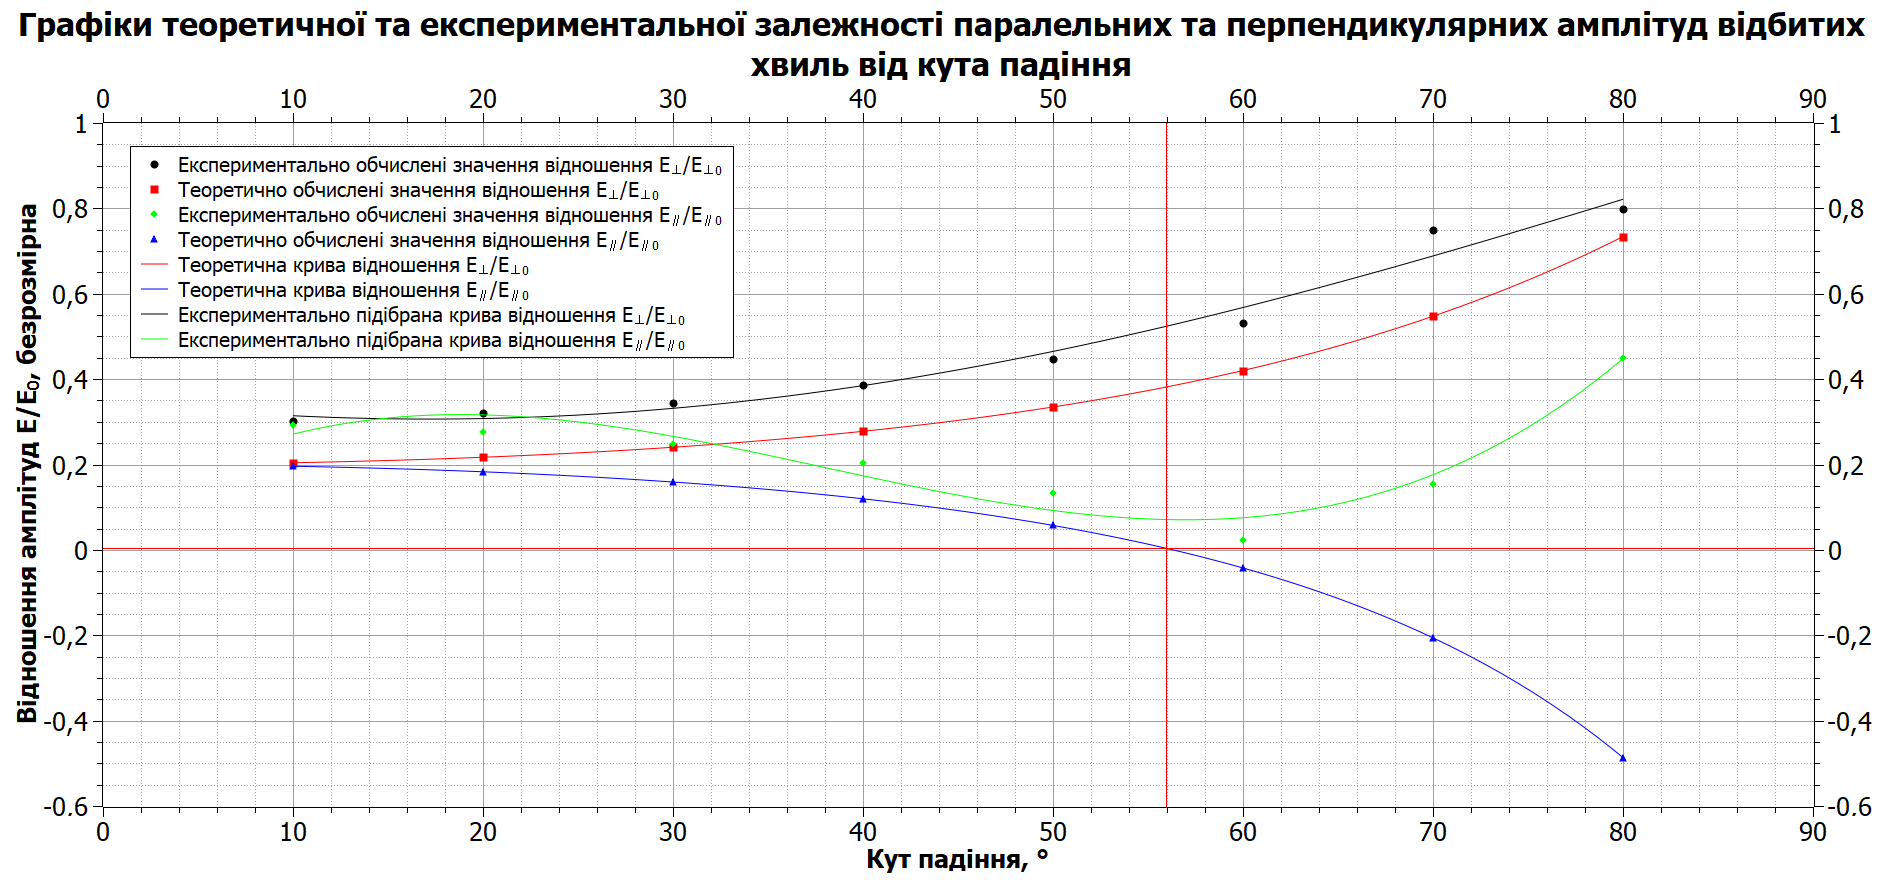
\includegraphics[width=0.7\textwidth]{graph1.png}
  \end{figure}

  Примітка. $E_{\parallel}$ може набувати від'ємних значень через фазовий зсув на $180^{\circ}$, тож для графічного відображення амплітуд без урахування фази беруть модуль.
  Фотодетектор реєструє лише інтенсивність $I \propto |E|^2 $, тому знак амплітуди не впливає на вимірювану величину.
  Також так як під час вимірювання величини $U$ я користувався кроком в 10 градусів, і "оминув" \ той кут, при якому експериментальне значення дорівнює 0, тому
  гіпотетичну пряму, при якій експериментальне значення відношень паралельних амплітуд я проведу на основі 0 в теоретичній кривій, і вийшов кут, близько
  $\vartheta_{\text{Бр}} \approx 57^{\circ}$. Звідси відоме відношення кута Брюстера:

  \[
  \tg \vartheta_{\text{Бр}} = n_2/n_1
  \]

\end{document}